% questions.tex —— 2012 年·陕西卷·理科 · 题目内容片段（无答案）
% 由 tools/generate_projects.py 依来源总账自 2012/2012_数学真题_陕西理_试题.md 生成，勿手改（改源 MD 后重跑）

\gkpart{一、选择题}

\begin{question}
\gkti{1}集合 $M=\{x\mid\lg x>0\}$，$N=\{x\mid x^2\leqslant4\}$，则 $M\cap N=$\mbox{（　　）}

（A）$(1,2)$；（B）$[1,2)$；（C）$(1,2]$；（D）$[1,2]$。

\end{question}
\begin{question}
\gkti{2}下列函数中，既是奇函数又是增函数的为\mbox{（　　）}

（A）$y=x+1$；（B）$y=-x^3$；（C）$y=\dfrac1x$；（D）$y=x|x|$。

\end{question}
\begin{question}
\gkti{3}设 $a$，$b\in\mathbf R$，$\mathrm i$ 是虚数单位，则“$ab=0$”是“复数 $a+\dfrac b{\mathrm i}$ 为纯虚数”的\mbox{（　　）}

（A）充分不必要条件；（B）必要不充分条件；（C）充分必要条件；（D）既不充分也不必要条件。

\end{question}
\begin{question}
\gkti{4}已知圆 $C:x^2+y^2-4x=0$，$l$ 是过点 $P(3,0)$ 的直线，则\mbox{（　　）}

（A）$l$ 与 $C$ 相交；（B）$l$ 与 $C$ 相切；（C）$l$ 与 $C$ 相离；（D）以上三个选项均有可能。

\Needspace{0.4\textheight}
\end{question}
\begin{question}
\gkti{5}如图，在空间直角坐标系中有直三棱柱 $ABC-A_1B_1C_1$，$CA=CC_1=2CB$，则直线 $BC_1$ 与直线 $AB_1$ 夹角的余弦值为\mbox{（　　）}
\nopagebreak[4]
\begin{center}% 2012 年陕西卷理科第 5 题：空间直角坐标系中的直三棱柱 ABC-A1B1C1。
% 来源 PDF：普通高考/2012/2012陕西理.pdf，第 1 页（印面 763）第 1 栏。
% 取 C(0,0,0)，A 沿 x 轴、B 沿 z 轴、C1 沿 y 轴；按原图取向作斜投影：
% x → (-0.8,-0.6)，y → (1.0,0.15)，z → (0,1)。
\begin{tikzpicture}[semithick, >=Stealth, font=\small]
  \coordinate (C)  at (0,0);
  \coordinate (A)  at (-1.6,-1.2);
  \coordinate (B)  at (0,1.4);
  \coordinate (C1) at (2.0,0.30);
  \coordinate (A1) at (0.4,-0.90);
  \coordinate (B1) at (2.0,1.70);
  % 坐标轴
  \draw[->] (0,0) -- (-2.0,-1.5) node[below] {$x$};
  \draw[->] (0,0) -- (0,1.9) node[left] {$z$};
  \draw[->] (0,0) -- (2.5,0.38) node[right] {$y$};
  % 棱柱
  \draw (C) -- (A) -- (B) -- cycle;
  \draw (A) -- (A1);
  \draw (C) -- (C1);
  \draw (B) -- (B1);
  \draw (A1) -- (B1);
  \draw (C1) -- (A1);
  \draw[dashed] (B1) -- (C1);
  \draw[dashed] (B) -- (C1);
  \draw (A) -- (B1);
  \node[below right] at (C) {$C$};
  \node[left] at (A) {$A$};
  \node[left] at (B) {$B$};
  \node[below right] at (C1) {$C_1$};
  \node[right] at (A1) {$A_1$};
  \node[above right] at (B1) {$B_1$};
\end{tikzpicture}
\end{center}
\nopagebreak[4]
（A）$\dfrac{\sqrt5}5$；（B）$\dfrac{\sqrt5}3$；（C）$\dfrac{2\sqrt5}5$；（D）$\dfrac35$。

\end{question}
\begin{question}
\gkti{6}从甲、乙两个城市分别随机抽取 $16$ 台自动售货机，对其销售额进行统计，统计数据用茎叶图表示（如图所示）。设甲、乙两组数据的平均数分别为 $\overline x_\text{甲}$，$\overline x_\text{乙}$，中位数分别为 $m_\text{甲}$，$m_\text{乙}$，则\mbox{（　　）}

\begin{center}
\begin{tabular}{lll}
\toprule
甲 & 茎 & 乙 \\
\midrule
$8$ $6$ $5$ & $0$ &  \\
$8$ $8$ $4$ $0$ $0$ & $1$ & $0$ $2$ $8$ \\
$7$ $5$ $2$ & $2$ & $0$ $2$ $3$ $3$ $7$ \\
$8$ $0$ $0$ & $3$ & $1$ $2$ $4$ $4$ $8$ \\
$3$ $1$ & $4$ & $2$ $3$ $8$ \\
\bottomrule
\end{tabular}
\end{center}

（A）$\overline x_\text{甲}<\overline x_\text{乙}$，$m_\text{甲}>m_\text{乙}$；（B）$\overline x_\text{甲}<\overline x_\text{乙}$，$m_\text{甲}<m_\text{乙}$；（C）$\overline x_\text{甲}>\overline x_\text{乙}$，$m_\text{甲}>m_\text{乙}$；（D）$\overline x_\text{甲}>\overline x_\text{乙}$，$m_\text{甲}<m_\text{乙}$。

\end{question}
\begin{question}
\gkti{7}设函数 $f(x)=x\mathrm e^x$，则\mbox{（　　）}

（A）$x=1$ 为 $f(x)$ 的极大值点；（B）$x=1$ 为 $f(x)$ 的极小值点；（C）$x=-1$ 为 $f(x)$ 的极大值点；（D）$x=-1$ 为 $f(x)$ 的极小值点。

\end{question}
\begin{question}
\gkti{8}两人进行乒乓球比赛，先赢 $3$ 局者获胜，决出胜负为止，则所有可能出现的情形（各人输赢局次的不同视为不同情形）共有\mbox{（　　）}

（A）$10$ 种；（B）$15$ 种；（C）$20$ 种；（D）$30$ 种。

\end{question}
\begin{question}
\gkti{9}在 $\triangle ABC$ 中，角 $A$，$B$，$C$ 所对边的长分别为 $a$，$b$，$c$，若 $a^2+b^2=2c^2$，则 $\cos C$ 的最小值为\mbox{（　　）}

（A）$\dfrac{\sqrt3}2$；（B）$\dfrac{\sqrt2}2$；（C）$\dfrac12$；（D）$-\dfrac12$。

\Needspace{0.4\textheight}
\end{question}
\begingroup
\renewenvironment{question}{\Needspace{0.5\textheight}}{}
\begin{question}
\gkti{10}如图所示是用模拟方法估计圆周率 $\pi$ 值的程序框图，$P$ 表示估计结果，则图中空白框内应填入\mbox{（　　）}
\nopagebreak[4]
\begin{center}% 2012 年陕西卷理科第 10 题：用模拟方法估计 π 的程序框图。
% 来源 PDF：普通高考/2012/2012陕西理.pdf，第 1 页（印面 763）第 2 栏。
% 流程：M=0,N=0,i=1 → 产生 x_i,y_i → x_i^2+y_i^2≤1? 是：M=M+1；否：N=N+1 →
%       i=i+1 → i>1000? 是：P=____ 后输出 P；否：回到产生随机数。
\begin{tikzpicture}[scale=0.86, transform shape, semithick, >=Stealth,
  block/.style={draw, minimum width=3.4cm, minimum height=0.62cm, align=center},
  wide/.style={draw, text width=7.6cm, minimum height=0.62cm, align=center},
  dec/.style={draw, diamond, aspect=2.6, inner sep=1pt, align=center},
  term/.style={draw, rounded corners=6pt, minimum width=1.5cm, minimum height=0.52cm},
  arr/.style={->}]
  \node (start) [term] at (0,9.0) {开始};
  \node (init)  [block] at (0,8.0) {$M=0,\ N=0,\ i=1$};
  \node (gen)   [wide, below=0.55cm of init] {产生两个 $0\sim1$ 之间的随机数 $x_i$，$y_i$};
  \node (dec)   [dec, below=0.75cm of gen] {$x_i^2+y_i^2\leqslant1$?};
  \node (m)     [block, right=0.9cm of dec] {$M=M+1$};
  \node (n)     [block, left=0.9cm of dec] {$N=N+1$};
  \node (inc)   [block, below=1.0cm of dec] {$i=i+1$};
  \node (dec2)  [dec, below=0.75cm of inc] {$i>1000$?};
  \node (p)     [block, below=0.8cm of dec2] {$P=\underline{\hspace{3.0em}}$};
  \node (out)   [block, below=0.5cm of p] {输出 $P$};
  \node (end)   [term, below=0.5cm of out] {结束};
  \draw[arr] (start) -- (init);
  \draw[arr] (init) -- (gen);
  \draw[arr] (gen) -- (dec);
  \draw[arr] (dec) -- node[above] {是} (m);
  \draw[arr] (dec) -- node[above] {否} (n);
  \draw[arr] (m) |- (inc.east);
  \draw[arr] (n) |- (inc.west);
  \draw[arr] (inc) -- (dec2);
  \draw[arr] (dec2) -- node[right] {是} (p);
  \draw[arr] (dec2.east) -- node[above] {否} ++(5.0,0) |- (0,7.45);
  \draw[arr] (p) -- (out);
  \draw[arr] (out) -- (end);
\end{tikzpicture}
\end{center}
\nopagebreak[4]
（A）$P=\dfrac N{1000}$；（B）$P=\dfrac{4N}{1000}$；（C）$P=\dfrac M{1000}$；（D）$P=\dfrac{4M}{1000}$。

\end{question}
\endgroup
\gkpart{二、填空题}

\begin{question}
\gkti{11}观察下列不等式：
\nopagebreak[4]
\[1+\frac1{2^2}<\frac32,\qquad1+\frac1{2^2}+\frac1{3^2}<\frac53,\qquad1+\frac1{2^2}+\frac1{3^2}+\frac1{4^2}<\frac74,\ \cdots\]
照此规律，第五个不等式为\gkblank{}。

\end{question}
\begin{question}
\gkti{12}$(a+x)^5$ 展开式中 $x^2$ 的系数为 $10$，则实数 $a$ 的值为\gkblank{}。

\Needspace{0.4\textheight}
\end{question}
\begin{question}
\gkti{13}如图是抛物线形拱桥，当水面在 $l$ 时，拱顶离水面 $2$ 米，水面宽 $4$ 米，水位下降 $1$ 米后，水面宽\gkblank{}米。
\nopagebreak[4]
\begin{center}% 2012 年陕西卷理科第 14 题：抛物线形拱桥，水面宽 4 米时拱顶离水面 2 米。
% 来源 PDF：普通高考/2012/2012陕西理.pdf，第 1 页（印面 765）第 3 栏。
\begin{tikzpicture}[scale=0.8, semithick]
  % 拱桥外形（抛物线 y = 2 - x^2/2 的拱顶向上）
  \draw[thick, domain=-2.6:2.6, samples=80] plot (\x, {2-(\x*\x)/2});
  % 两侧桥体
  \fill[pattern=north east lines] (-2.6,0) -- (-2.6,-1.2) -- (2.6,-1.2) -- (2.6,0) -- cycle;
  \draw (-2.6,0) -- (-2.6,-1.2) -- (2.6,-1.2) -- (2.6,0);
  % 水面
  \draw[thick] (-2.6,-0.0) -- (2.6,-0.0);
  % 水位标注
  \draw[<->] (-3.0,0) -- (-3.0,2) node[midway,left] {$2\ \mathrm m$};
  \draw[<->] (-2,-1.5) -- (2,-1.5) node[midway,below] {$4\ \mathrm m$};
\end{tikzpicture}
\end{center}
\nopagebreak[4]
\end{question}
\begin{question}
\gkti{14}设函数 $f(x)=\begin{cases}\ln x,&x>0,\\-2x-1,&x\leqslant0,\end{cases}$ $D$ 是由 $x$ 轴和曲线 $y=f(x)$ 及该曲线在点 $(1,0)$ 处的切线所围成的封闭区域，则 $z=x-2y$ 在 $D$ 上的最大值为\gkblank{}。

\Needspace{0.4\textheight}
\end{question}
\begin{question}
\gkti{15}三选一。

【A】若存在实数 $x$ 使 $|x-a|+|x-1|\leqslant3$ 成立，则实数 $a$ 的取值范围是\gkblank{}。

【B】如图，在圆 $O$ 中，直径 $AB$ 与弦 $CD$ 垂直，垂足为 $E$，$EF\perp DB$，垂足为 $F$。若 $AB=6$，$AE=1$，则 $DF\cdot DB=$\gkblank{}。
\nopagebreak[4]
\begin{center}% 2012 年陕西卷理科第 15B 题：圆 O 中直径 AB 与弦 CD 垂直，垂足 E，EF⊥DB 于 F。
% 来源 PDF：普通高考/2012/2012陕西理.pdf，第 1 页（印面 765）第 3 栏。
\begin{tikzpicture}[scale=0.9, semithick, every node/.style={inner sep=1.5pt}]
  \coordinate (O) at (0,0);
  \draw (O) circle (2.4);
  \coordinate (A) at (-2.4,0);
  \coordinate (B) at (2.4,0);
  \draw (A) -- (B);
  \coordinate (E) at (-0.8,0);
  \coordinate (C) at (-0.8,2.263);
  \coordinate (D) at (-0.8,-2.263);
  \draw (C) -- (D);
  \draw (B) -- (D);
  \coordinate (F) at ($(D)!0.62!(B)$);
  \draw (E) -- (F);
  \node[left] at (A) {$A$};
  \node[right] at (B) {$B$};
  \node[above] at (C) {$C$};
  \node[below] at (D) {$D$};
  \node[above] at (E) {$E$};
  \node[right] at ([xshift=2pt]F) {$F$};
  \node[below right] at (O) {$O$};
\end{tikzpicture}
\end{center}
\nopagebreak[4]
【C】直线 $2\rho\cos\theta=1$ 与圆 $\rho=2\cos\theta$ 相交的弦长为\gkblank{}。

\end{question}
\gkpart{三、解答题}

\begin{question}
\gkti{16}函数 $f(x)=A\sin\left(\omega x-\dfrac\pi6\right)+1$（$A>0$，$\omega>0$）的最大值为 $3$，其图象相邻两条对称轴之间的距离为 $\dfrac\pi2$。

（1） 求函数 $f(x)$ 的解析式；

（2） 设 $\alpha\in\left(0,\dfrac\pi2\right)$，$f\left(\dfrac\alpha2\right)=2$，求 $\alpha$ 的值。

\end{question}
\begin{question}
\gkti{17}设 $\{a_n\}$ 是公比不为 $1$ 的等比数列，其前 $n$ 项和为 $S_n$，且 $a_5$，$a_3$，$a_4$ 成等差数列。

（1） 求数列 $\{a_n\}$ 的公比；

（2） 证明：对任意 $k\in\mathbf N_+$，$S_{k+2}$，$S_k$，$S_{k+1}$ 成等差数列。

\Needspace{0.4\textheight}
\end{question}
\begin{question}
\gkti{18}（1） 如图，证明命题“$a$ 是平面 $\pi$ 内的一条直线，$b$ 是 $\pi$ 外的一条直线（$b$ 不垂直于 $\pi$），$c$ 是直线 $b$ 在 $\pi$ 上的投影，若 $a\perp b$，则 $a\perp c$”为真；

（2） 写出上述命题的逆命题，并判断其真假（不需证明）。
\nopagebreak[4]
\begin{center}% 2012 年陕西卷理科第 18 题：平面 π 内的直线 a，π 外的直线 b 及其投影 c。
% 来源 PDF：普通高考/2012/2012陕西理.pdf，第 2 页（印面 764）第 1 栏。
% 斜二测画平面 π 为平行四边形；b 从平面上方斜穿，c 为其在 π 上的投影。
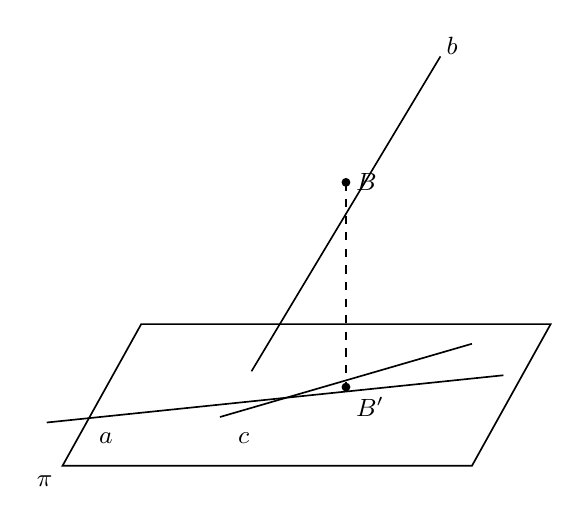
\begin{tikzpicture}[semithick, font=\small]
  % 平面 π
  \draw (0,0) -- (5.2,0) -- (6.2,1.8) -- (1.0,1.8) -- cycle;
  \node[below left] at (0,0) {$\pi$};
  % 直线 a（在平面内）
  \draw (-0.2,0.55) -- (5.6,1.15);
  \node[below] at (0.55,0.55) {$a$};
  % 投影 c（在平面内）
  \coordinate (B) at (3.6,3.6);
  \coordinate (Bp) at (3.6,1.0);
  \draw (2.0,0.62) -- (5.2,1.55);
  \node[below] at (2.3,0.55) {$c$};
  % 直线 b 及垂线 BB'
  \draw (2.4,1.2) -- (4.8,5.2);
  \node[above right] at (4.75,5.1) {$b$};
  \draw[dashed] (B) -- (Bp);
  \fill (Bp) circle (1.6pt);
  \node[below right] at (Bp) {$B'$};
  \fill (B) circle (1.6pt);
  \node[right] at (B) {$B$};
\end{tikzpicture}
\end{center}
\nopagebreak[4]
\end{question}
\begin{question}
\gkti{19}已知椭圆 $C_1:\dfrac{x^2}4+y^2=1$，椭圆 $C_2$ 以 $C_1$ 的长轴为短轴，且与 $C_1$ 有相同的离心率。

（1） 求椭圆 $C_2$ 的方程；

（2） 设 $O$ 为坐标原点，点 $A$，$B$ 分别在椭圆 $C_1$ 和 $C_2$ 上，$\overrightarrow{OB}=2\overrightarrow{OA}$，求直线 $AB$ 的方程。

\end{question}
\begin{question}
\gkti{20}某银行柜台设有一个服务窗口，假设顾客办理业务所需的时间互相独立，且都是整数分钟，对以往顾客办理业务所需的时间统计结果如下：

\begin{center}
\begin{tabular}{llllll}
\toprule
办理业务所需的时间（分） & $1$ & $2$ & $3$ & $4$ & $5$ \\
\midrule
频率 & $0.1$ & $0.4$ & $0.3$ & $0.1$ & $0.1$ \\
\bottomrule
\end{tabular}
\end{center}

从第一个顾客开始办理业务时计时。

（1） 估计第三个顾客恰好等待 $4$ 分钟开始办理业务的概率；

（2） $X$ 表示至第 $2$ 分钟末已办理完业务的顾客人数，求 $X$ 的分布列及数学期望。

\end{question}
\begin{question}
\gkti{21}设函数 $f_n(x)=x^n+bx+c$（$n\in\mathbf N_+$，$b$，$c\in\mathbf R$）。

（1） 设 $n\geqslant2$，$b=1$，$c=-1$，证明：$f_n(x)$ 在区间 $\left(\dfrac12,1\right)$ 内存在唯一零点；

（2） 设 $n=2$，若对任意 $x_1$，$x_2\in[-1,1]$，有 $|f_2(x_1)-f_2(x_2)|\leqslant4$，求 $b$ 的取值范围；

（3） 在（1）的条件下，设 $x_n$ 是 $f_n(x)$ 在 $\left(\dfrac12,1\right)$ 内的零点，判断数列 $x_2$，$x_3$，$\cdots$，$x_n$，$\cdots$ 的增减性。

\end{question}